\pagebreak
\subsubsection{UC49-Avvia chat}
\begin{figure}[h] 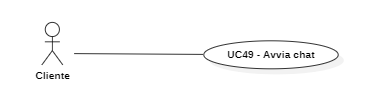
\includegraphics[scale=1]{uc49.png} \end{figure}
\begin{itemize}
\item \textbf{Attore principale:} Cliente.
\item \textbf{Precondizioni:} Il cliente è nella pagina di visualizzazione di un ristorante.
\item \textbf{Postcondizioni:} Diventa possibile comunicare con il ristoratore.
\item \textbf{Scenario principale:}
\begin{enumerate}
    \item Il cliente ha dei dubbi che vuole chiarire;
    \item Il cliente seleziona la funzionalità di avvio della chat;
    \item Il sistema crea la chat;
    \item Diventa possibile comunicare bidirezionalmente tra il cliente e il ristoratore.
\end{enumerate}
\end{itemize}

\subsubsection{UC50-Visualizzazione lista chat}
\begin{figure}[h] 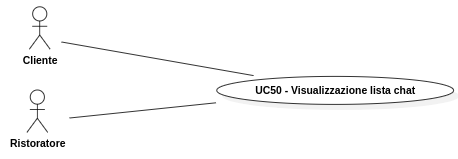
\includegraphics[scale=1]{uc50.png} \end{figure}
\begin{itemize}
\item \textbf{Attore principale:} Cliente / Ristoratore.
\item \textbf{Precondizioni:} L'utente sta visualizzando la propria dashboard.
\item \textbf{Postcondizioni:} L'utente visualizza le possibili chat con cui interagire.
\item \textbf{Scenario principale:}
\begin{enumerate}
    \item L'utente seleziona la funzionalità di visualizzazione della chat.
    \item L'utente visualizza l'elenco di chat avviate;
    \item Per ogni chat vengono visualizzate le seguenti informazioni:
      \begin{itemize}
        \item Il nome profilo dell'altra parte;
        \item La timestamp dell'ultimo messaggio inviato;
        \item I primi 20 caratteri dell'ultimo messaggio inviato.
\item L'utente può selezionare una chat per interagire con essa (si veda UC51).
      \end{itemize}
\end{enumerate}
\end{itemize}

\pagebreak

\subsubsection{UC51-Apertura chat}
\begin{figure}[h] 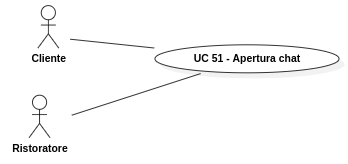
\includegraphics[scale=1]{uc51.png} \end{figure}
\begin{itemize}
\item \textbf{Attore principale:} Cliente / Ristoratore.
\item \textbf{Precondizioni:} L'utente sta visualizzando la lista di chat interagibili.
\item \textbf{Postcondizioni:} L'utente visualizza la cronologia dei messaggi.
\item \textbf{Scenario principale:}
\begin{enumerate}
    \item L'utente seleziona chat con cui vuole interagire.
    \item L'utente visualizza la cronologia di messaggi inviati o ricevuti in ordine temporale decrescente;
    \item Per ogni messaggio vengono visualizzate le seguenti informazioni:
      \begin{itemize}
        \item Il nome del profilo del mittente;
        \item La timestamp del messaggio;
        \item Il contenuto testuale del messaggio.
      \end{itemize}
\end{enumerate}
\end{itemize}

\subsubsection{UC52-Invio messaggio}
\begin{figure}[h] 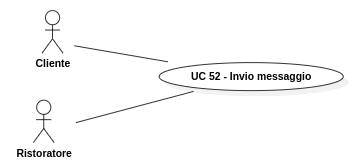
\includegraphics[scale=1]{uc52.png} \end{figure}
\begin{itemize}
\item \textbf{Attore principale:} Cliente / Ristoratore
\item \textbf{Precondizioni:} È stata aperta la chat.
\item \textbf{Postcondizioni:} È stato inviato il messaggio.
\item \textbf{Scenario principale:}
\begin{enumerate}
    \item L'attore principale scrive il messaggio nella barra di testo messa a disposizione;
    \item L'attore conferma l'invio;
    \item Il messaggio viene salvato dal sistema in forma criptata;
    \item Il destinatario riceve il messaggio.
\end{enumerate}
\end{itemize}
